\question[5] En la Figura \ref{ondas}, se encuentra un diagrama representativo de un comportamiento ondulatorio. Completa los espacios en blanco con la propiedad de las ondas a la que se refiere:
    \begin{figure}[H]
        \centering
        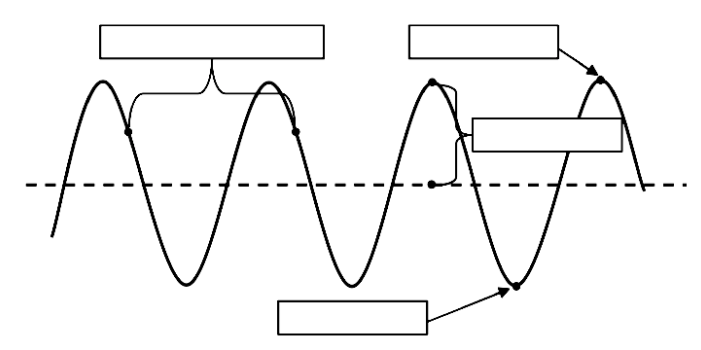
\includegraphics[width =0.5\textwidth ]{Images/onda_blanco.png}
        \caption{Diagrama gen\'erico de una onda y algunas de sus caracter\'isticas.}
        \label{ondas}
    \end{figure}